\section{Theorie}
\label{sec:theorie}

Ein Operationsverstärker ist definiert als ein elektronischer Verstärker, der gleichspannungsgekoppelt ist und einen hohen Verstärkungsfaktor besitzt.
Er kann benutzt werden, um verschiedene mathematische Rechenoperationen durchzuführen, wie Addieren, Subtrahieren, Differenzieren und Integrieren.\\
Der ideale Operationsverstärker hat zwei Eingänge und einen verstärkenden Ausgang, der unabhängig von äußeren Einflüssen einen gleichbleibenden Verstärkungsfaktor ohne Verluste besitzt.
Das Schaltzeichen dafür ist in \autoref{fig:symbol} dargestellt.

\begin{figure}[H]
    \centering
    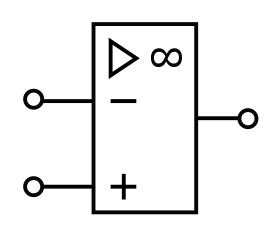
\includegraphics[scale=0.5]{images/symbol.png}
    \caption{Darstellung eines Operationsverstärkers nach DIN-EN-6067 Norm.\cite{V51}}
    \label{fig:symbol}
\end{figure}

Bei einem invertierenden Linearverstärker, dessen Schaltung in \autoref{fig:linear} dargestellt ist, beträgt der ideale Verstärkungsfaktor somit
\begin{equation}
    V_{theo} = -\frac{R_2}{R_1}
    \label{eq:verstaerkung}
\end{equation}

\begin{figure}[H]
    \centering
    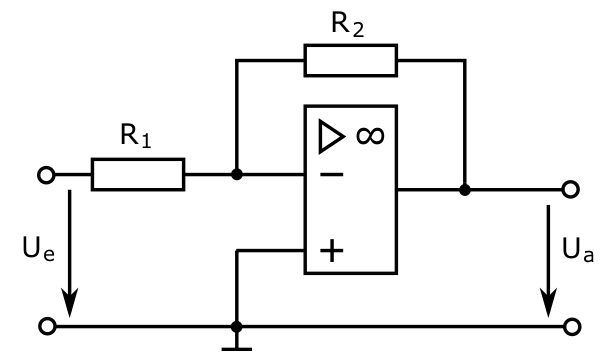
\includegraphics[scale=0.5]{images/linear.png}
    \caption{Aufbau eines invertierenden linearen Verstärkers.\cite{V51}}
    \label{fig:linear}
\end{figure}

Alle realen Operationsverstärker besitzen zusätzlich zum positiven und negativen Eingang noch zwei Eingänge für die Versorgungsspannung.
Diese werden typischerweise mit $U_{+}$ und $U_{-}$ bezeichnet.\\
Dabei ist es wichtig die Versorgungsspannung symmetrisch zu wählen, da diese das Ausgangssignal beeinflusst.
Der Operationsverstärker besitzt eine Saturierungsspannung, die vorgibt, wie hoch $U_{out}$ in Abhängigkeit von $U_{+,-}$ sein kann.
In \autoref{fig:satur} ist das graphisch dargestellt.

\begin{figure}[H]
    \centering
    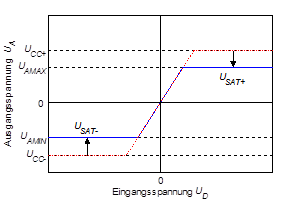
\includegraphics[]{images/satur.png}
    \caption{Dieser Graph zeigt den Verlauf der Ausgangsspannung bei anliegender Eingangsspannung in Abhängigkeit der Versorgungsspannung an.
    Es ist zu erkennen, dass die Saturierungsspannung $U_{SAT}$ die Ausgangsspannung abhängig von der Versorgungsspannung betragsmäßig verringert.\cite{satur}}
    \label{fig:satur}
\end{figure}

Die Formel zur Berechnung der Ausgangsspannung ist:
\begin{equation}
    \begin{aligned}
        U_{out,max} = U_{+} - U_{SAT+}\\
        U_{out,min} = U_{-} - U_{SAT-}
    \end{aligned}
\end{equation}
Daraus geht hervor, dass eine unsymmetrische Versorgungsspannung zu einer unsymmetrischen Ausgangsspannung führt, was für einen Betrieb mit Wechselspannung unerwünschte Effekte zur Folge hat.\\

\subsection{Invertierender Linearverstärker}
Der invertierende Linearverstärker wurde bereits in \autoref{fig:linear} dargestellt.
Hierbei wird der Operationsverstärker bei einer Parallel-Spannungs-Gegenkopplung betrieben.
Die Verstärkung ist nicht konstant, wie bei einem idealen Verstärker, sondern nimmt bei steigender Frequenz der Eingangsspannung ab.
Der Übergang von konstanter Verstärkung zu abfallender Verstärkung ist ab der Grenzfrequenz $f_{Grenz}$ erkennbar.\\
Die Leerlaufverstärkung lässt sich durch die Relation
\begin{equation}
    V' = \frac{U_{out}}{U_{in}}
    \label{eq:ampli}
\end{equation}
bestimmen.\\
Damit ist die Bandbreite mittels $B=f_{Grenz}\cdot \bar{V'}$ gegeben, wobei $\bar{V'}$ der Mittelwert der Verstärkung $V'$ ist.

\subsection{Umkehr-Integrierer und invertierender Differenzierer}
Die Schaltung des Umkehr-Integrierers ist ähnlich aufgebaut, wie die des Linearverstärkers.
Statt des zweiten Widerstands wird jedoch ein Kondensator verbaut.\\
Aus den primären Verhältnissen
\begin{equation}
    \begin{aligned}
        U_{in} = R\cdot I_{in}\\
        U_{out} = U_C = \frac{1}{C}\int I_C dt
    \end{aligned}
\end{equation}
wird das mathematische Verhältnis des Integrierers berechnet.
Es gilt die Relation:
\begin{equation}
    U_{out} = -\frac{1}{RC}\int U_{in} dt
    \label{eq:integrierer}
\end{equation}
Die Proportionalität beträgt demnach $-\frac{1}{RC}$.\\
\newline
Bei der Schaltung des invertierenden Differenzierers werden Widerstand und Kondensator vom Umkehr-Integrierer vertauscht.
Die dabei geltenden Verhältnisse sind
\begin{equation}
    \begin{aligned}
        I_{in} = \dot{Q} = C\cdot \dot{U}_{in}\\
        U_{out} = R\cdot I_{out}.
    \end{aligned}
\end{equation}
Das sich daraus ergebende Verhältnis ist \autoref{eq:diff}.
\begin{equation}
    U_{out} = -RC\cdot \dot{U}_{in}
    \label{eq:diff}
\end{equation}
Hierbei ist die Proportionalität $-RC$.

\subsection{Nicht-Invertierender Schmitt-Trigger}
Die Schaltung des nicht-invertierenden Schmitt-Triggers ist ähnlich aufgebaut zum invertierenden Linearverstärker, mit dem Unterschied, dass, wie in \autoref{fig:schmitt} dargestellt, der invertierende Eingang auf Masse liegt.
Das hat einen Schalter-Effekt zur Folge, der ab einer bestimmten Eingangspannung schaltet, die Schwellspannung genannt wird.
In \autoref{fig:hysterese} ist das Verhalten von Ein- und Ausgangsspannung des Schmitt-Triggers dargestellt.

\begin{figure}[H]
    \centering
    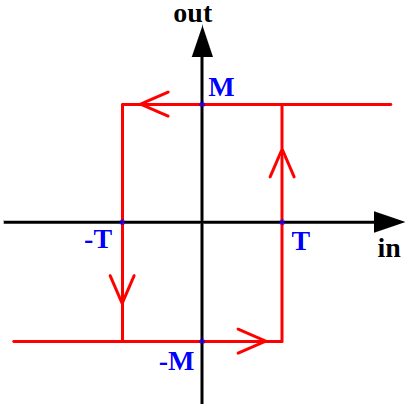
\includegraphics[scale=0.5]{images/hysterese.png}
    \caption{Kennlinie des Schmitt-Triggers mit eingezeichneter Schwellspannung T.\cite{schmitt}}
    \label{fig:hysterese}
\end{figure}

Der theoretische Wert für die Schwellspannung berechnet sich aus den verwendeten Widerständen und beträgt:
\begin{equation}
    T = \frac{R_1}{R_1 + R_2}\cdot U_{max}
    \label{eq:schmitt}
\end{equation}
$U_{max}$ ist dabei die maximale Ausgangsspannung.

\subsection{Signalgenerator}
Der Signalgenerator Aufbau ist in \autoref{fig:signal} dargestellt.\\
An dieser Schaltung liegt keine Eingangsspannung an, doch durch die Rückkopplung des Integrierers auf den Schmitt-Trigger wird eine Schwingung induziert, die eine Dreiecksform aufweist.
Die Frequenz und Amplitude dieser Schwingung berechnen sich aus den Komponenten der Schaltung und ergeben die Gleichungen in \ref{eq:signal}.
\begin{equation}
    \begin{aligned}
        f_{\Delta} = \frac{R_2}{4CR_1R_3}\\
        \text{und}\\
        A = \frac{R_1}{R_2}\cdot U_{max}
    \end{aligned}
    \label{eq:signal}
\end{equation}
Durch Veränderung der Komponenten lassen sich so verschiedene Signale generieren.